%% 
%% Copyright 2007-2020 Elsevier Ltd
%% 
%% This file is part of the 'Elsarticle Bundle'.
%% ---------------------------------------------
%% 
%% It may be distributed under the conditions of the LaTeX Project Public
%% License, either version 1.2 of this license or (at your option) any
%% later version.  The latest version of this license is in
%%    http://www.latex-project.org/lppl.txt
%% and version 1.2 or later is part of all distributions of LaTeX
%% version 1999/12/01 or later.
%% 
%% The list of all files belonging to the 'Elsarticle Bundle' is
%% given in the file `manifest.txt'.
%% 
%% Template article for Elsevier's document class `elsarticle'
%% with harvard style bibliographic references

\documentclass[authoryear,preprint,12pt]{elsarticle}

%% The `ecrc' package must be called to make the CRC functionality available
%\usepackage{ecrc}

%% Use the option review to obtain double line spacing
%% \documentclass[authoryear,preprint,review,12pt]{elsarticle}

%% Use the options 1p,twocolumn; 3p; 3p,twocolumn; 5p; or 5p,twocolumn
%% for a journal layout:
%% \documentclass[final,1p,times,authoryear]{elsarticle}
%% \documentclass[final,1p,times,twocolumn,authoryear]{elsarticle}
%% \documentclass[final,3p,times,authoryear]{elsarticle}
%% \documentclass[final,3p,times,twocolumn,authoryear]{elsarticle}
%% \documentclass[final,5p,times,authoryear]{elsarticle}
%% \documentclass[final,5p,times,twocolumn,authoryear]{elsarticle}

%% For including figures, graphicx.sty has been loaded in
%% elsarticle.cls. If you prefer to use the old commands
%% please give \usepackage{epsfig}

%% The amssymb package provides various useful mathematical symbols
\usepackage{amssymb}
%% The amsthm package provides extended theorem environments
%% \usepackage{amsthm}

%% The lineno packages adds line numbers. Start line numbering with
%% \begin{linenumbers}, end it with \end{linenumbers}. Or switch it on
%% for the whole article with \linenumbers.
%% \usepackage{lineno}

\journal{Applied Mathematical Modelling}

\begin{document}

\begin{frontmatter}
%% Title, authors and addresses

%% use the tnoteref command within \title for footnotes;
%% use the tnotetext command for theassociated footnote;
%% use the fnref command within \author or \affiliation for footnotes;
%% use the fntext command for theassociated footnote;
%% use the corref command within \author for corresponding author footnotes;
%% use the cortext command for theassociated footnote;
%% use the ead command for the email address,
%% and the form \ead[url] for the home page:
%% \title{Title\tnoteref{label1}}
%% \tnotetext[label1]{}
%% \author{Name\corref{cor1}\fnref{label2}}
%% \ead{email address}
%% \ead[url]{home page}
%% \fntext[label2]{}
%% \cortext[cor1]{}
%% \affiliation{organization={},
%%            addressline={}, 
%%            city={},
%%            postcode={}, 
%%            state={},
%%            country={}}
%% \fntext[label3]{}

\title{Multi-product Batch Processing Time Maximization Problem}

%% use optional labels to link authors explicitly to addresses:
%% \author[label1,label2]{}
%% \affiliation[label1]{organization={},
%%             addressline={},
%%             city={},
%%             postcode={},
%%             state={},
%%             country={}}
%%
%% \affiliation[label2]{organization={},
%%             addressline={},
%%             city={},
%%             postcode={},
%%             state={},
%%             country={}}

%\author{Tatiana Balbi Fraga, Ítalo Ruan Barbosa de Aquino and Regilda da Costa e Silva Menêzes}

\author{Tatiana Balbi Fraga\corref{cor1}\fnref{label1}}
\ead{tatiana.balbi@ufpe.br}
\cortext[cor1]{corresponding author}

\author{Ítalo Ruan Barbosa de Aquino\fnref{label1}}
\ead{italo_ruan_@hotmail.com}

\author{Regilda da Costa e Silva Menêzes\fnref{label1}}
\ead{regilda.smenezes@ufpe.br}

%\affiliation[label1]{
%			 organization={Centro Acadêmico do Agreste - Universidade Federal de Pernambuco},
%             addressline={Avenida Marielle Franco, Bairro Nova Caruaru},
%             city={Caruaru},
%             postcode={55014-900},
%             state={PE},
%             country={Brasil} }

\affiliation[label1]{
		   organization={Agreste Academic Center - Federal University of Pernambuco},%Department and Organization
           addressline={Avenida Marielle Franco, Nova Caruaru}, 
           city={Caruaru},
           postcode={55014-900}, 
           state={PE},
           country={Brazil}}

\begin{abstract}
In the plastic bag extrusion process, it is necessary to determine the optimal processing time for batches formed by different products, which are processed simultaneously by the same extruder, but with different processing rates. The batch processing time must be determined in order to meet a series of known constraints, such as the limitation for the quantity produced for each product and for the quantity produced for the set of all products in the same batch. In this paper we present this problem as a new combinatorial optimization problem named Multi-product Batch Processing Time Maximization (MPBPTM) problem. We also present a mathematical model for the MPBPTM problem and an analytical solution method with polynomial time complexity, which proved to be able to obtain optimal solutions for several benchmarks in a very short time, even for very large instances.
\end{abstract}
%%Graphical abstract
\begin{graphicalabstract}
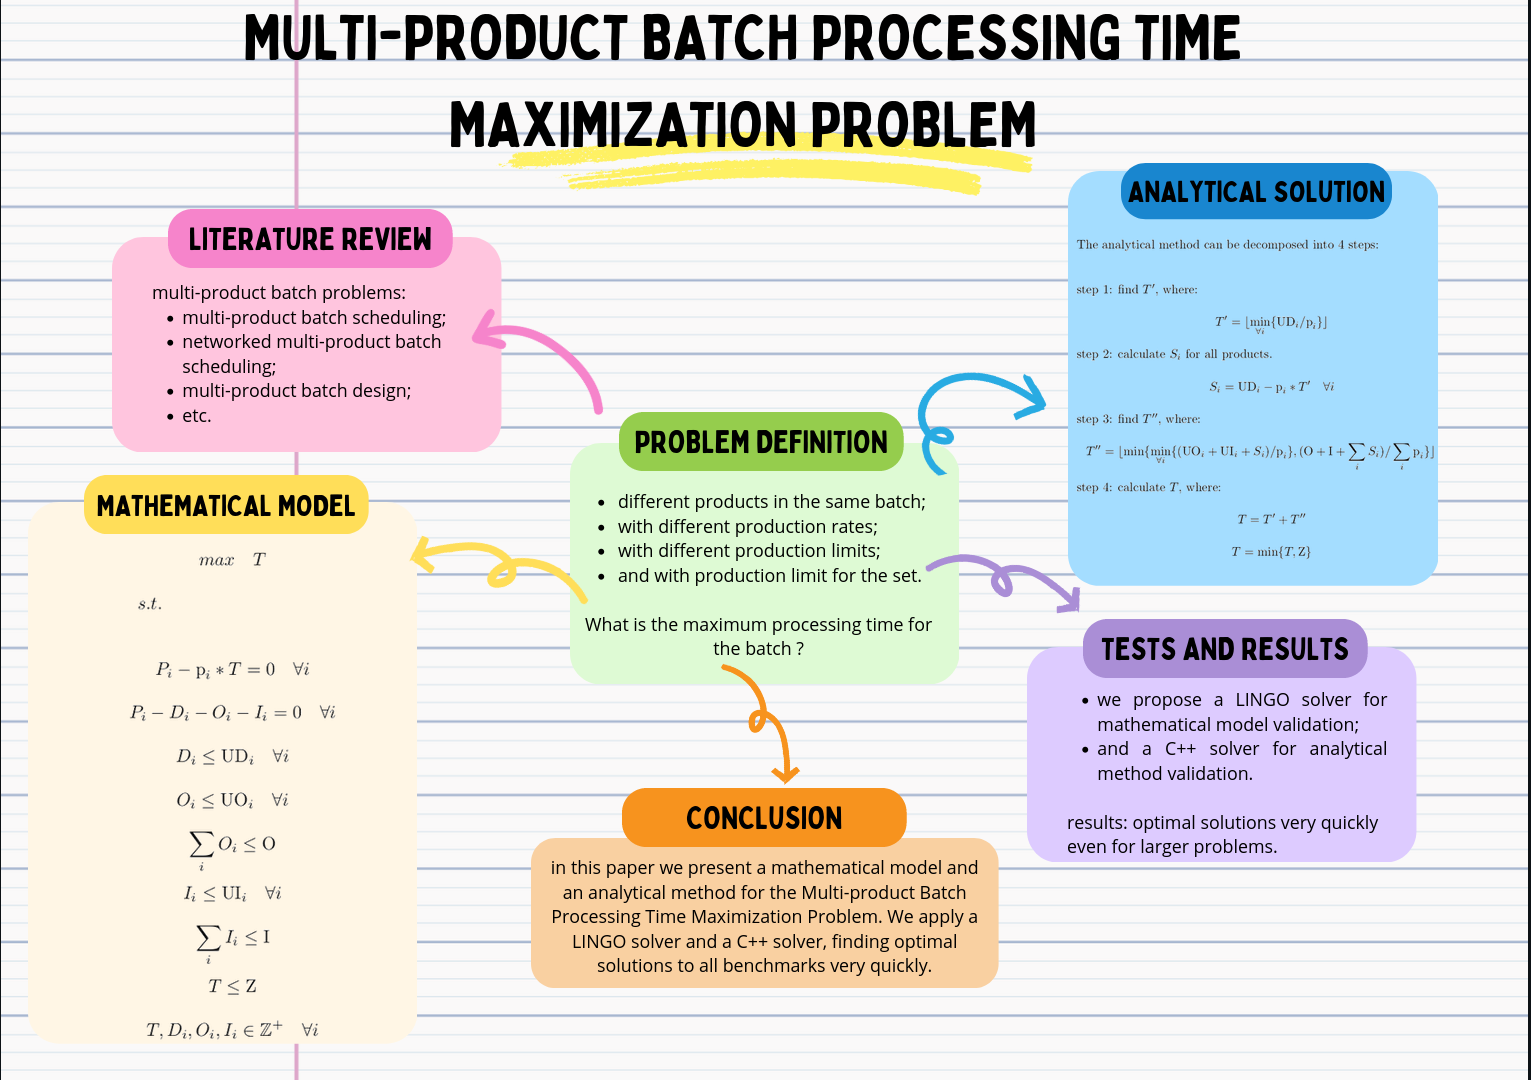
\includegraphics[width=0.8\textwidth]{graphical.png}
\end{graphicalabstract}

%%Research highlights
\begin{highlights}
\item brief bibliographic review on multi-product batch problems;
\item new combinatorial optimization problem named Multi-product Batch Processing Time Maximization (MPBPTM) problem;
\item linear integer programming model for the MPBPTM problem;
\item exact optimization method for solving the MPBPTM problem.
\end{highlights}

\begin{keyword}
multiproduct batch \sep processing time maximization \sep analytical solution \sep C++ \sep LINGO
\end{keyword}
\end{frontmatter}

%% \linenumbers

%% main text
\section{Introduction}
\label{sec:intro}

The scientific literature presents several papers that address multi-product batch problems. Many works target the problem of multi-product batch scheduling (MPBS), in which it is necessary to determine the production sequence of the products and the ideal batch size for each product, in a production of several products which share the same production facilities and for which demand is known \citep{Eilon1985}. In this problem, a single product is processed at a time, so it is necessary that the quantity produced is sufficient to meet the demand during the period in which other products are being processed. The solution must be determined in such a way that both setup and storage costs are minimized. Among the authors who addressed this problem are \cite{Eilon1985}, \cite{Omega1993} and \cite{LiuEtAl2020}. \cite{MendezEtAll2000} and \cite{ShiEtAll2017} present two parallel multi-product batch scheduling (PMPBS) problems, in which production units of the same type are arranged in parallel, forming each production stage. In this case, it is also necessary to define in which units each product will be processed. The authors also take into account other constraints for the problem (\emph{e.g.}, release time and due date for the products, and sequencing constraints due to mismatched product colors sequences) and other goals (\emph{i.e.}, optimize customer satisfaction and/or the plant performance). In the papers mentioned above, production in a single unit or in a serial flowshop plant is considered, in which all products follow a linear flow through the production stages. \cite{KimEtAl1996} consider the multi-product batch problem in networked processes. As defined by the authors, in this case, the production units are not arranged in lines, and the connection between the units may or may not exist. Therefore, the production paths in the flowshop network can be different for each product. Also the passing of previous batch can be possible so that the final sequence of the production at the last stage units can be different from the initial sequence. In all papers presented above, each batch contains only one product type, and each machine can process only one batch (or product type) at a time. \cite{LiEtAl2022} deal with a PMPBS problem involving incompatible families with different job sizes and capacity constraints. In this problem, solutions are accepted in which two or more batches are processed simultaneously on the same machine. However, there are no production limitations for the production of each product group. The paper of \cite{LiEtAl2022} also presente an extensive literature review on production batch scheduling problems. Other important works deal with the problem of a multi-product batch plant design (MPBPD). In this case the problem is to obtain the configuration of the plant and the equipment that minimize the capital cost of all the equipment items needed to fulfill the production requirements (Ravemark and Rippin, 1998).

In this work, we are concerned with determining the ideal processing time for a single batch consisting of a set of products, each product being or not different from the other products of the same batch. That is, we consider a specific case where different products are processed simultaneously on the same processor. This case occurs, for example, during the processing of plastic bags in extruders, where the resins are melted, then pass through a cylinder forming a balloon and this balloon, after cooling, is stored in a coil which, in turn, is cut into several smaller coils with different models of plastic bags.

As scientific contributions, in this paper we define a new multi-product batch problem, named multi-product batch processing time maximization (MPBPTM) problem, as well as a mathematical model and a polynomial time complexity analytical solution optmization method for solving this problem.

In the next sections, a presentation of problem is made along with an application example. Section \ref{sec:mathModel} presents an interger linear mathematical model for the problem and section \ref{sec:analyticalSol} presents an analytical method for its solution. Section \ref{sec:results} presents the tests and results obtained by a solver in C++ applying the analytical solution and a solver developed in LINGO to new proposed benchmarks. In sections \ref{sec:contributions} and \ref{sec:acknowledgments}, the contributions to this work are informed and acknowledgments are given, respectively. Finally, section \ref{sec:conclusions} presents the paper's conclusions and suggestions for future works.

\section{Multi-product batch processing time maximization problem}
\label{sec:MBPTMP}

The multi-product batch processing time maximization problem arises when a set of different products are processed simultaneously in a same production batch. In this problem, it is considered that the quantity produced of each product is directly proportional to the processing time, however, with a different constant of proportionality (production rate) for each product. In addition, there is a maximum quantity allowed for the production of batch products, defined both individually and for the set. The maximum production quantity of each product is mainly defined according to the demand for the product. However, it is still possible to stock the products and/or send them to the outlets. In both cases, there is a stocking/shipping limit for each product and a stocking/shipping limit for the set of products in the batch. Also, there is a time limit available for processing the batch. The problem consists of defining the maximum processing time for the batch, respecting the limitations related to the quantities produced. For a better understanding of the problem, an example is presented below.

\emph{Example:} A certain machine must process a batch containing 2 different products: A and B. The production rate of A is 60 g/min while the production rate of B is 40 g/min. The factory has free stock for a maximum of 3000 g of any product, and, according to the company's inventory policy, a maximum of 3000 g of product A and 2000 g of product B can be stocked at the factory. There is a demand for 1000 g of product A and 500 g of product B. The factory has an outlet that has free space in stock of 1000 g, which can receive a maximum of 600 g of each product. A maximum time of 100 minutes of this machine can be allocated for processing this batch. What is the maximum possible time for processing this batch ? 

\section{Mathematical model}
\label{sec:mathModel}

Given that: \\

$\textrm{UD}_i$ is the demand for the product $i$;

$\textrm{I}$ is the maximum quantity allowed for additional factory storage of all products in the batch;

$\textrm{UI}_i$ is the maximum quantity allowed for stocking the product $i$ in the factory;

$\textrm{O}$ is the maximum quantity allowed for shipment of all products to outlets;

$\textrm{UO}_i$ is the maximum amount of product $i$ that can be shipped to outlets;

$\textrm{p}_i$ is the production rate of product $i$;

$\textrm{Z}$ is the timeout for batch processing;

$P_i$ is the amount of product $i$ produced;

$D_i$ is the amount of product $i$ delivered for the demand;

$O_i$ amount of product $i$ shipped to factory outlets;

$I_i$ is the amount of product $i$ that will be stored at the factory;

$T$ is the batch processing time. \\

We have the problem: \\

\begin{equation}
max \quad T
\end{equation}

$s.t.$

\begin{equation}
P_i - \textrm{p}_i * T  = 0 \quad \forall i
\end{equation}

\begin{equation}
P_i - D_i - O_i - I_i = 0 \quad \forall i
\end{equation}

\begin{equation}
D_i \leq \textrm{UD}_i \quad \forall i
\end{equation}

\begin{equation}
O_i \leq \textrm{UO}_i \quad \forall i
\end{equation}

\begin{equation}
\sum_i{O_i} \leq \textrm{O}
\end{equation}

\begin{equation}
I_i \leq \textrm{UI}_i \quad \forall i
\end{equation}

\begin{equation}
\sum_i{I_i} \leq \textrm{I}
\end{equation}

\begin{equation}
T \leq \textrm{Z}
\end{equation}

\begin{equation}
T, D_i, O_i, I_i \in  \mathbb{Z}^+ \quad \forall i
\end{equation}

where: \\

Constraints in (2) relate the quantity produced, $P_i$, to batch processing time $T$. Constraints in (3) calculate the quantity produced, $P_i$, as a function of the primary variables, $D_i$, $O_i$ and $I_i$. Constraints in (4), (5), and (7) state that the quantity delivered to demand, the quantity shipped to the autlets, and the factory-stocked quantity of each product must be less than their respective known limits. Constraints (6) and (8) state that both the sum of product quantities sent to the autlets and the sum of product quantities stocked in the factory must be less than their respective maximum allowed values. The restriction in (9) establishes that there is a batch processing time limit, $\textrm{Z}$, that must be respected. And finally, the constraints in (10) inform the nature of the decision variables.



\section{Analytical solution}
\label{sec:analyticalSol}

It is possible to consider the factory stock and the outlets stock as single stock, so we have:

\begin{equation}
E_i = O_i + I_i
\end{equation}

where $E_i$ is the sum of the quantity stored at the factory and the quantity sent to the outlets of the product $i$. \\

So that:

\begin{equation}
E_i \leq \textrm{UO}_i + \textrm{UI}_i
\end{equation}

and

\begin{equation}
\sum_i {E_i} \leq \textrm{O} + \textrm{I}
\end{equation}


It is also possible to split the batch processing time into two time slots:

\begin{equation}
T = T' + T''
\end{equation}

and consider that $T'$ is the maximum processing time used only for production that will meet the demand. Thus, we can find $T'$, solving the reduced problem:

\begin{equation}
max \quad T'
\end{equation}

$s.t.$

\begin{equation}
D_i - \textrm{p}_i * T'  = 0 \quad \forall i
\end{equation}

\begin{equation}
D_i \leq \textrm{UD}_i \quad \forall i
\end{equation}

\begin{equation}
D_i, T' \in  \mathbb{Z}^+ \quad \forall i
\end{equation}

This reduced problem can be rewritten in the form:

\begin{equation}
max \quad T'
\end{equation}

$s.t.$ \\

\begin{equation}
T'  \leq \lfloor{\textrm{UD}_i / \textrm{p}_i}\rfloor \quad \forall i
\end{equation}

So we have that $T'$ will be the smallest of the ratios $\lfloor{\textrm{UD}_i / \textrm{p}_i}\rfloor$ of all products. \\

Once we find the value of $T'$, we can calculate the value of unmet demand for each product after $T'$, $S_i$, through the equations in (\ref{eq:unmet1}).

\begin{equation}
\label{eq:unmet1}
S_i = \textrm{UD}_i - \textrm{p}_i * T' \quad \forall i
\end{equation}

Now we consider that the time interval $T''$ will be used for the production of the quantities that will be stored (in the factory and in the outlets), as well as of the demand not met by the production in the first time interval, $S_i$. 

In this case, we can find $T'''$ by solving the second reduced problem:

\begin{equation}
max \quad T''
\end{equation}

$s.t.$

\begin{equation}
E_i - \textrm{p}_i * T''  = 0 \quad \forall i
\end{equation}

\begin{equation}
E_i - S_i \leq \textrm{UO}_i + \textrm{UI}_i \quad \forall i
\end{equation}

\begin{equation}
\sum_i {E_i - S_i} \leq \textrm{O} + \textrm{I}
\end{equation}

\begin{equation}
E_i, T'' \in  \mathbb{Z}^+ \quad \forall i
\end{equation}

Again, using a little algebra, we can rewrite this reduced problem in the form:

\begin{equation}
max \quad T''
\end{equation}

$s.t.$

\begin{equation}
T'' \leq \lfloor{(\textrm{UO}_i + \textrm{UI}_i + S_i) / \textrm{p}_i}\rfloor  \quad \forall i
\end{equation}

\begin{equation}
T'' \leq \lfloor{(\textrm{O} + \textrm{I} + \sum_i {S_i}) / \sum_i {\textrm{p}_i}}\rfloor
\end{equation}

So, being $\textrm{N}$ the number of products in the batch, we will have $\textrm{N}+1$ inequalities that limit the value of $T''$ by constants and again $T''$ will be defined by the smallest value. \\

So, the analytical method can be decomposed into 4 steps: \\

step 1: find $T'$, where:
\begin{equation}
T' = \lfloor{\min_{\forall i} \{\textrm{UD}_i / \textrm{p}_i\}}\rfloor
\end{equation}

step 2: calculate $S_i$ for all products.
\begin{equation}
\label{eq:unmet}
S_i = \textrm{UD}_i - \textrm{p}_i * T' \quad \forall i
\end{equation}

step 3: find $T''$, where:
\begin{equation}
T'' = \lfloor{\min \{\min_{\forall i} \{(\textrm{UO}_i + \textrm{UI}_i + S_i) / \textrm{p}_i\},(\textrm{O} + \textrm{I} + \sum_i {S_i}) / \sum_i {\textrm{p}_i}\}}\rfloor
\end{equation}

step 4: calculate $T$, where: 
\begin{equation}
T = T' + T''
\end{equation}
\begin{equation}
T = \min \{T , \textrm{Z}\}
\end{equation}

It is probably possible to extend this thinking to the solution of a class of linear optimization problems. However, we will work on this concept in an upcoming paper. \\

\emph{Solution for the example presented before} \\

Applying the method for solving the example presented in section \ref{sec:MBPTMP}, we have: \\

$T' \leq \lfloor{1000 \textrm{ g} / (60 \textrm{ g}/\textrm{min})}\rfloor$ \\

$T' \leq 16 \textrm{ min}$ \quad for A \\

$T' \leq \lfloor{500 \textrm{ g} / (40 \textrm{ g}/\textrm{min})}\rfloor$ \\

$T' \leq 12 \textrm{ min}$ \quad for B \\

so: \\

$T' = 12 \textrm{ min}$ \\

Then:\\

$S_A = 1000 \textrm{ g} - 12 \textrm{ min} * 60 \textrm{ g}/\textrm{min} = 280 \textrm{ g}$ \\

$S_B = 500 \textrm{ g} - 12 \textrm{ min} * 40 \textrm{ g}/\textrm{min} = 20 \textrm{ g}$ \\

And so we have: \\

$T'' \leq \lfloor{(3000 \textrm{ g} + 600 \textrm{ g} + 280 \textrm{ g}) / (60 \textrm{ g}/\textrm{min})}\rfloor$ \\

$T'' \leq 64 \textrm{ min}$ \quad for A \\

$T'' \leq \lfloor{(2000 \textrm{ g} + 600 \textrm{ g} + 20 \textrm{ g}) / (40 \textrm{ g}/\textrm{min})}\rfloor$ \\

$T'' \leq 65 \textrm{ min}$ \quad for B \\

$T'' \leq \lfloor{(1000 \textrm{ g} + 3000 \textrm{ g} + 300 \textrm{ g}) / (100 \textrm{ g}/\textrm{min})}\rfloor$ \\

$T'' \leq 43 \textrm{ min}$ \quad for A and B \\

So that: \\

$T'' = 43 \textrm{ min}$ \\

So we have: \\

$T = 55 \textrm{ min}$ \\

As $T<\textrm{Z}$, then $T = 55 \textrm{ min}$ will certainly be the optimal solution. \\

In this case we will have: \\

$P_A = 3300 \textrm{ g}$ e $P_B=2200 \textrm{ g}$ \\

$D_A = 1000 \textrm{ g}$ e $D_B = 500 \textrm{ g}$ \\

$E_A = 2300 \textrm{ g}$ e $E_B = 1700 \textrm{ g}$ \\

Note that it is not important to know the values of $O_i$ and $I_i$, $\forall i$, however, after determining a solution, these values can be found by taking a solution from the undetermined system of inequalities:

\begin{equation}
O_i + I_i = E_i \quad \forall i
\end{equation}

\begin{equation}
O_i \leq \textrm{UO}_i \quad \forall i
\end{equation}

\begin{equation}
\sum_i{O_i} \leq \textrm{O}
\end{equation}

\begin{equation}
I_i \leq \textrm{UI}_i \quad \forall i
\end{equation}

\begin{equation}
\sum_i{I_i} \leq \textrm{I}
\end{equation}

\begin{equation}
O_i, I_i \in  \mathbb{Z}^+ \quad \forall i
\end{equation}

\section{Tests and results}
\label{sec:results}

To test the developed model and analytical solution method, we created a solver in C++ and a solver in LINGO (https://github.com/tbfraga/COPSolver). The tests were performed on a notebook with an Intel i7 processor. We tested the solvers developed for the benchmarks presented on Tables \ref{tab:MBPTMP001}, \ref{tab:MBPTMP002} and \ref{tab:MBPTMP003}, and for randon benchmarks generated by the following functions: \\

\begin{equation}
\textrm{p}_i = \textrm{rand}()\%30 + 10
\end{equation}

\begin{equation}
\textrm{UD}_i = \textrm{rand}()\%3000 + 800;
\end{equation}

\begin{equation}
 \textrm{seed1} = \textrm{rand}()\%3000 + 500;
\end{equation}

\begin{equation}
\textrm{seed2} = \textrm{rand}()\%5000 + 1000;
\end{equation}

\begin{equation}
\textrm{O} = \textrm{N}/2*\textrm{seed1};
\end{equation}

\begin{equation}
\textrm{UO}_i = \textrm{rand}()\%(\textrm{seed1}-500) + 500;
\end{equation}

\begin{equation}
\textrm{I} = \textrm{N}/2*\textrm{seed2};
\end{equation}

\begin{equation}
\textrm{UI}_i = \textrm{rand}()\%(\textrm{seed2}-1000) + 1000;
\end{equation}

\begin{equation}
\textrm{Z} = 100;
\end{equation}


\begin{table}[h]
\begin{center}
\begin{tabular}[c]{c r r r}
$i$ & 1 & 2 & total \\
\cline {1-4} \\
$\textrm{p}_i$ & 60 & 40 & \\
$\textrm{UD}_i$ & 1000 & 500 & \\
$\textrm{UO}_i$ & 600 & 600 & 1000 \\
$\textrm{UI}_i$ & 3000 & 2000 & 3000 \\
\cline {1-4} \\
& & $\textrm{Z}$ & 100 \\
\end{tabular}
\caption{Benchmark MPBPTMP 001}
\label{tab:MBPTMP001}
\end{center}
\end{table}

\begin{table}[h]
\begin{center}
\begin{tabular}[c]{c r r r r}
$i$ & 1 & 2 & 3 & total \\
\cline {1-5} \\
$\textrm{p}_i$ & 60 & 40 & 50 \\
$\textrm{UD}_i$ & 1000 & 500 & 800 \\
$\textrm{UO}_i$ & 600 & 600 & 600 & 1500 \\
$\textrm{UI}_i$ & 3000 & 2000 & 1000 & 3500 \\
\cline {1-5} \\
& & & $\textrm{Z}$ & 100 \\
\end{tabular}
\caption{Benchmark MPBPTMP 002}
\label{tab:MBPTMP002}
\end{center}
\end{table}

\begin{table}[h]
\begin{center}
\begin{small}
\begin{tabular}[c]{c r r r r r r r r r r r }
$i$ & 1 & 2 & 3 & 4 & 5 & 6 & 7 & 8 & 9 & 10 & total \\
\cline {1-12} \\
$\textrm{p}_i$ & 60 & 40 & 50 & 40 & 30 & 50 & 60 & 10 & 20 & 40\\
$\textrm{UD}_i$ & 1000 & 500 & 800 & 500 & 400 & 500 & 2000 & 300 & 500 & 1000 \\
$\textrm{UO}_i$ & 600 & 600 & 600 & 1500 & 300 & 200 & 500 & 800 & 0 & 200 & 3000 \\
$\textrm{UI}_i$ & 3000 & 2000 & 1000 & 800 & 3000 & 1000 & 400 & 300 & 200 & 0 & 5000 \\
\cline {1-12} \\
& & & & & & & & & & $\textrm{Z}$ & 100 \\
\end{tabular}
\caption{Benchmark MPBPTMP 003}
\label{tab:MBPTMP003}
\end{small}
\end{center}
\end{table}

Randomly generated benchmarks were named RMPBPTMP $\textrm{N}$, being $\textrm{N}$ the number of products. Seeking to enable the reproduction of the results, in the computational construction of the benchmarks we used the function srand((unsigned) source), where source is a defined value. To build the results presented in this work, we used source=0. The benchmarks used for the tests performed can be consulted at github.com/blinded.

Table \ref{tab:results} presents the results obtained by applying the analytical method (C++ solver) and the LINGO solver for the solution of the previously presented benchmarks.

\begin{table}[h]
\begin{center}
\begin{footnotesize}
\begin{tabular}[c]{l r r r r}
problem & LINGO solver & time (s) & analytical method & time (s) \\
\cline {1-5} \\
MPBPTMP 1 & 55 & 0.04 & 55 & 0.001 \\
MPBPTMP 2 & 48 & 0.06 & 48 & 0.001 \\
MPBPTMP 3 & 30 & 0.09 & 30 & 0.001 \\
RMPBPTMP 20 & 100 & 0.08 & 100 & 0.001 \\
RMPBPTMP 50 & 98 & 0.12 & 98 & 0.001\\
RMPBPTMP 100 & 98 & 0.12 & 98 & 0.002\\
RMPBPTMP 1,000 & 78 & 3.10 & 78 & 0.002\\
RMPBPTMP 10,000 & 70 & 168.87 & 70 & 0.006 \\
\cline {1-5} \\
\end{tabular}
\caption{Results obtained with the LINGO solver and the analytical method}
\label{tab:results}
\end{footnotesize}
\end{center}
\end{table}

It is important to point out that the LINGO solver was developed with the purpose of validating the results found by the proposed analytical method. As the analytical method is a polynomial time complexity method, we did not intend to compare computational costs, however it is possible to verify that both solvers are capable of finding optimal solutions for the proposed benchmarks very quickly, even for very large problems.

We have considered here a one-day period problem, so in a future work we will study the complexities of solving a multi-period problem and try to propose new solution methods if needed. 

\section{Conclusions and suggestions for future works}
\label{sec:conclusions}

In this paper we presented the Multi-product Batch Processing Time Maximization problem, as well as a mathematical model and an analytical solution method for this problem. The mathematical model and analytical method were tested, respectively, by a solver developed with the LINGO software, from LINDO Systems, and with a solver developed in C++ language. Optimum results were found for all proposed benchmarks, very quickly, even in the case of very large problems, which demonstrates the efficiency of the proposed method. As in this paper we considered a planning period of one day, in a future work we will study the complexities that arise when considering the same problem in a multi-period scenario. We will also verify if there is the possibility of extending the proposed analytical method to solve a class of linear integer programming problems with similar characteristics to the studied problem.

\section{CRediT authorship contribution statement} 
\label{sec:contributions}

T.B. Fraga: Conceptualization, Project administration, Supervision, Software, Methodology, Validation, Formal analysis, Writing – original draft, Writing – review \& editing. Í.R.B. Aquino: Data curation. R.C.S. Menêzes: Data curation.

\section{Acknowledgments}
\label{sec:acknowledgments}

We are enormously grateful to Coordenação de Aperfeiçoamento de Pessoal de Nível Superior (CAPES) and to Conselho Nacional de Desenvolvimento Científico e Tecnológico (CNPq) for the financial support provided to our projects. We also thank LINDO systems team for the LINGO software license, without which this work would not have been possible and the to the owner of the company in the plastics sector, who allowed us to learn about his company's production process. Finally, we would like to thank Pró-reitoria de Extensão e Cultura da UFPE (PROExC) and the Research Director of Propesqi (Pró-reitoria de Pesquisa e Inovação da UFPE) for their support and recognition of our work, and dear Professors Antônio José da Silva Neto and João Flávio Vieira de Vasconcellos from IPRJ/UERJ, who contributed significantly to the formation of essential skills for the development of our projects. We also thank my co-worker Marcos Luiz Henrique, for having helped by evaluating the mathematical model and solution method proposed in this paper.

%% The Appendices part is started with the command \appendix;
%% appendix sections are then done as normal sections
%% \appendix

%% \section{}
%% \label{}

%% If you have bibdatabase file and want bibtex to generate the
%% bibitems, please use
%%
%%  \bibliographystyle{elsarticle-harv} 
%%  \bibliography{<your bibdatabase>}

%% else use the following coding to input the bibitems directly in the
%% TeX file.

\begin{thebibliography}{1}

%% \bibitem[Author(year)]{label}
%% Text of bibliographic item

\bibitem[\protect\citeauthoryear{Eilon}{1985}]{Eilon1985}
Eilon. (1985). Multi-product batch production on a single machine - A problem revisited. {\it OMEGA Int. J. of Mgmt Sci.}, Vol. 13 (5), pp. 453--468.

\bibitem[\protect\citeauthoryear{Kim \emph{et al.}}{1996}]{KimEtAl1996}
Kim, M., Jung, J. H. and Lee, I. (1996). Intelligent scheduling and monitoring for multi-product networked batch processes. {\it  Computers chem. Engn}, Vol. 20 (Suppl.), pp. 1149--1154.

\bibitem[\protect\citeauthoryear{Li et al.}{2022}]{LiEtAl2022}
Li, C., Wang, F., Gupta, J.N.D., Chung, T. (2022). Scheduling identical parallel batch processing machines involving incompatible families with different job sizes and capacity constraints. {\it Computers \& Industrial Engineering}, Vol. 169, pp. 108115.

\bibitem[\protect\citeauthoryear{Liu \emph{et al.}}{2020}]{LiuEtAl2020}
Liu, G., Li, F., Yang, X., and Qiu. S. (2020). The multi-stage multi-product batch-sizing problem in the steel industry. {\it  Applied Mathematics and Computation}, Vol. 369, 124830.

\bibitem[\protect\citeauthoryear{Méndez \emph{et al.}}{2000}]{MendezEtAll2000}
Méndez, C.A., Henning, G.P., Cerdá, J. (2000). Optimal scheduling of batch plants satisfying multiple product
orders with different due-dates. {\it Computers and Chemical Engineering}, Vol. 24, pp. 2223--2245.

\bibitem[\protect\citeauthoryear{Omega Journal}{1993}]{Omega1993}
OMEGA Journal. (1993). Single Machine Multi-product Batch Scheduling: Testing Several Solution Methods. {\it  OMEGA Int. J. of Mgmt Sci.}, Vol. 21 (6), pp. 709--711.

\bibitem[\protect\citeauthoryear{Ravemark and Rippin}{1998}]{RavemarkAndRippin1998}
Ravemark, D. E., and Rippin, D. W. T. (1998). Optimal design of a multi-product batch plant. {\it Computers chem. Engng}, Vol. 22 (1-2), pp. 177--183.

\bibitem[\protect\citeauthoryear{Shi \emph{et al.}}{2017}]{ShiEtAll2017}
Shi, B., Qian, X., Sun, S., Yan, L. (2017). Rule-based scheduling of multi-stage multi-product batch plants with parallel units. {\it Chinese Journal of Chemical Engineering}, in press.

\end{thebibliography}
\end{document}

\endinput
%%
%% End of file `elsarticle-template-harv.tex'.
